% !TEX root = ../dnn_ba.tex
\chapter{Der verwendete Datensatz}
\label{chap:datensatz}

Dieses Kapitel beleuchtet den in der Forschungsarbeit verwendeten Datensatz. Hierfür wird zunächst erläutert, welche Eigenschaften der Datensatz erfüllen muss, damit die Ergebnisse der Arbeit auf die praktische Anwendung übertragbar sind. Im Zuge dessen werden die Anforderungen aufgelistet und es wird kurz erläutert, wie diese durch den vorliegenden Datensatz erfüllt werden.
Weiterhin wird auf die Aufzeichnung und Merkmalsextraktion des Datensatzes eingegangen, die darin enthaltenen Klassen vorgestellt und die aus dem Zeitbereich extrahierten Merkmale im Detail besprochen.

\section{Anforderungen an den Datensatz}

Der Prozess der Klassifikation und Zuordnung eines EMG-Signals zur dazugehörigen Bewegung kann in drei Schritte unterteilt werden:

\begin{itemize}
	\item die \textbf{\textit{Merkmalsextraktion}},
	\item die \textbf{\textit{Dimensionsreduktion}}
	\item und die \textbf{\textit{Musterklassifikation}}
\end{itemize}

Während man sich in der Praxis mit der Optimierung aller drei Phasen beschäftigen muss, liegt der Fokus dieser Arbeit auf der Musterklassifikation eines bereits durch \cite{Kaufmann2013Data} präparierten Datensatzes. Da daher die nachträgliche Manipulation der Merkmalsextraktion und Dimensionsreduktion ausgeschlossen ist, müssen im vorliegenden Datensatz einige Eigenschaften vorliegen, um eine Übertragbarkeit der hier erzielten Ergebnisse auf die Praxisanwendung sicherzustellen.

Die erste Anforderung ist die Extraktion der Merkmale unter möglichst geringer Rechenintensität. Da die Klassifikation von Muskelaktivität in ES Anwendung findet, die aufgrund ihrer physischen Eigenschaften häufig keine hohe Rechenleistung besitzen (\cite{Allard2019}), muss die Rechenintensität der angewandten Algorithmen den Anforderungen dieser Systeme entsprechen. Hierfür muss entschieden werden, ob die Merkmale aus dem Zeit- oder Frequenzbereich extrahiert werden. Während die Merkmalsextraktion aus dem Frequenzbereich oder einer Mischung aus Frequenz- und Zeitbereich Vorteile in der Rauschreduktion mit sich bringt, ist sie im Vergleich zur Extraktion der Merkmale aus dem Zeitbereich rechnerisch intensiv (\cite{zecca2002control}) und daher schlechter geeignet für die Nutzung in ES. Der verwendete Datensatz enthält mit den Merkmalen des \textit{mean absolute value}, des \textit{zero crossings}, des \textit{slope sign changes} und der \textit{waveform length} vier Merkmale des Zeitbereichs (\cite{Kaufmann2013Data}), weshalb davon ausgegangen werden kann, dass die Merkmale rechnerisch effizient extrahiert werden können. Auf die Eigenschaften der extrahierten Merkmale wird im folgenden Abschnitt weiter eingegangen.

Desweiteren ist es nach \cite{Engelhart2003} für die Übertragbarkeit in praktische Anwendungsfälle notwendig, den gesamten Prozess der Merkmalsextraktion, Dimensionsreduktion und Musterklassifikation innerhalb eines kleinen Zeitfensters zu vollenden. Dieses ist in der Regel etwa 300 Millisekunden groß. Systeme, die diese Zeitschwelle überschreiten, könnten in der Anwendung eine kognitiv wahrnehmbare Verzögerung zwischen Anweisung (Muskelkontraktion) und Durchführung aufweisen, was zu erheblichen Einschränkungen in der Nutzbarkeit durch den Anwender resultieren könnte (\cite{Engelhart2003}). Im vorliegenden Datensatz wurden Zeitfenster von jeweils 150 Millisekunden an aufgezeichneten Daten für jede einzelne Klassifikation verwendet (\cite{Kaufmann2013Data}). Das bedeutet, dass die verbleibenden 150 Millisekunden für die Klassifikation genutzt werden können. Ein solches Zeitfenster erweist sich mit Blick auf bisherige Untersuchungen als ausreichend (\cite{Engelhart2003}), um die maximale Verzögerung von 300 Millisekunden nicht zu überschreiten.

Ein letztes Merkmal ist außerdem eine ausreichende Datenmenge. Vorige Untersuchungen in dem Gebiet zeigten bereits auf, dass inetwa fünf Trainings-Durchläufe notwendig sind, um eine hohe Klassifikationsgenauigkeit zu erzielen (\cite{Kaufmann2013}).  Der Datensatz wurde vom Probanden über einen Zeitraum von 21 Tagen mit jeweils fünf bis sechs Einheiten am Tag aufgezeichnet. Insgesamt enthält der Datensatz 121 Aufzeichungen.  Somit kann anhand vorgehender Untersuchungen abgeleitet werden, dass eine hohe Klassifikationsgenauigkeit bereits durch Training mit einem der 21 aufgezeichneten Tage erreicht werden kann (\cite{Kaufmann2013Data}).

\section{Aufzeichnung des Datensatzes}
\label{sec:datensatz-aufnahme}

\begin{figure}[h]
	\begin{center}
	\includegraphics[scale=0.17]{grafiken/electrode-positioning.jpg}
	\caption{Position der Elektroden am Unterarm (\cite{Kaufmann2013Data})}
	\label{elektroden-position}
	\end{center}
\end{figure}
% Allgemeine Eigenschaften des Datensatzes (Zeitraum, Frequenz, Beschaffenheit der Daten)
Für das Erfassen der Daten wurde dem Proband im Rahmen der Forschung durch \cite{Kaufmann2013Data} ein tragbares Datenerfassungssystem mit vier EMG-Kanälen am Unterarm angelegt (Abbildung \ref{elektroden-position}). Dieses zeichnete die elektrischen Signale mit einer Auflösung von 24 bit und einer sampling rate von 2048 Hz auf. Dabei wurde die Position der Elektroden nach der ersten Aufzeichnung auf der Haut des Probanden markiert, um in folgenden Aufzeichnungen die Position replizieren zu können und so Ungenauigkeiten bei der Messung einzugrenzen. 

In jeder Aufnahmesitzung wurden mehrere Bewegungen in Folge erfasst. Jede Bewegung besteht dabei aus einer vier-sekündigen Entspannungs- und einer fünf-sekündigen Kontraktionsphase. Die Kontraktionsphase lässt sich dabei wiederum in eine ein-sekündige Anfangsphase und eine vier-sekündige stetige Phase unterteilen (\cite{Kaufmann2013Data}). 


\begin{figure}[h]
	\begin{center}
	\includegraphics[scale=0.4]{grafiken/feature-extraction.png}
	\caption{Merkmalsextraktion aus der stetigen Phase (\cite{Kaufmann2013Data})}
	\label{feature-extraction}
	\end{center}
\end{figure}

Wie in Abbildung \ref{feature-extraction} zu sehen ist, erfolgte die Merkmalsextraktion anhand des Signals in der stetigen Phase.
Dieser Abschnitt wird in Fenster von jeweils 150ms unterteilt, aus denen jeweils die Merkmale extrahiert werden. Anschließend wird das Fenster um 150ms verschoben. Auf diese Weise bleiben die Aufzeichnungen der Klassen untereinander differenzierbar und das Signal wird gleichzeitig um überschüssiges Rauschen bereinigt, um die rechnerische Intensität zu verringern (\cite{Kaufmann2013Data}). 


\begin{figure}[ht]
	\begin{center}
	\includegraphics[scale=0.5]{grafiken/11classes.png}
	\caption{Im Datensatz enthaltene Merkmale (\cite{Kaufmann2013Data})}
	\label{bewegungsklassen}
	\end{center}
\end{figure}


% Kurze Vorstellung der Merkmale
Der Datensatz enthält laut \cite{Kaufmann2013Data}, wie in Abbildung \ref{bewegungsklassen} zu sehen, elf gekennzeichnete Bewegungen des Handgelenks, die alle jeweils über den gesamten Aufzeichnungszeitraum erfasst wurden. Enthalten ist 1) die Streckung, 2) die Beugung, 3) die Ulnare Abduktion, 4) die Radiale Abduktion, 5) die Innenrotation, 6) die Außenrotation, 7) das Öffnen, 8) das Schließen, 9) der Schlüsselgriff, 10) der ''Pincher-Grip'' und 11) das Ausstrecken des Zeigefingers.

\section{Extrahierte Merkmale}

% Detaillierteres Eingehen auf die aus dem Zeitbereich extrahierten Merkmale
Aus den vier je Elektrode extrahierten Merkmalen entsteht somit eine Liste aus $4 * 4 = 16$ Merkmalen für jedes Fenster in der jeweiligen Aufzeichnung (\cite{Kaufmann2013Data}). Es handelt sich wie bereits im vorigen Kapiteln erwähnt um Merkmale aus dem Zeitbereich, die bereits in dem Papier von \cite{zecca2002control} detailliert beschrieben wurden und auf die nun im Folgenden weiter eingegangen wird.

Nach \cite{Engelhart2003} setzen sich die extrahierten Klassen wie folgt zusammen:

\textit{Mean Absolute Value (MAV)}:
Der Mean Absolute Value bildet den Durchschnittswert eines Signals $x$ über den Zeitraum $i$, der in Summe $L$ Signale enthält.

$$\bar{x}_i = \frac{1}{L}\sum_{k=1}^{L}|x_k|\;f\ddot{u}r\;i=1,...,I$$

\textit{zero crossings (ZC)}:
Zero Crossings geben an, wie häufig ein Signal die Nullmarke passiert. Um durch Rauschen ausgelöste Überschreitungen auszuschließen, wird dafür eine Schwelle $\varepsilon$ festgelegt. Vergleicht man also nun die zwei Punkte $x_k$ und $x_k+1$ im Verlauf des Signals, kann man die Anzahl der Nulldurchgänge um 1 erhöhen, wenn folgende Bedingungen gegeben sind:

$$\{x_k > 0 \;und\; x_{k+1} < 0\}\;oder\;\{x_k < 0\;und\;x_{k+1} > 0\}$$
$$|x_k - x_{k + 1}| \geq \varepsilon$$


\textit{slope sign changes (SSC)}:
Die Anzahl der slope sign changes, also der Vorzeichenwechsel der Steigung in einem aufgezeichneten Signal, werden ebenfalls als Merkmal verwendet. Sie funktionieren dahingehend ähnlich wie ZC, da hier ebenfalls jedes Mal, wenn ein aufgezeichnetes Signal die Schwelle $\varepsilon$ überschreitet, ein Zähler inkrementiert wird. Betrachtet werden dabei auf dem Signal die Punkte $x_{k - 1}$, $x_k$ und $x_{k+1}$. Inkrementiert wird unter folgenden Bedingungen:

$$\{x_k > x_{k-1}\;und\;x_k > x_{k+1}\}\;oder\;\{x_k < x_{k-1}\;und\;x_k<x_{k+1}\}$$
$$|x_k-x_{k+1}|\geq\varepsilon\;oder\;|x_k-x_{k-1}|\geq\varepsilon$$

\textit{waveform length (WL)}:
Die durch die nachfolgende Formel von \cite{Engelhart2003} beschriebene waveform length gibt die Signallänge des jeweiligen Aufnahmefensters an. Diese ergibt sich aus der kummulierten Differenz $\Delta{x_k}$ der Punkte $x_k$ und $x_{k-1}$ über die gesamte Summe der Signale L (\cite{Engelhart2003}).

$$l_0=\sum_{k=1}^{L}|\Delta{x_k}|$$

Nach erfolgter Extraktion werden die 16 erfassten Merkmale pro Zeitfenster zu einer Liste zusammengefügt. Das 17te Element der Liste kodiert dabei die in diesem Fenster aufgenommene Klasse, während das 18te Element die Aufnahmesitzung angibt. Dadurch entsteht eine Liste aus mit der jeweiligen Klasse und der Aufnahmesitzung kodierten Merkmalen (Abbildung \ref{dataset-item}), mit denen nun die Klassifikatoren trainiert werden können.
\bigskip
\begin{figure}[h]
	\begin{center}
		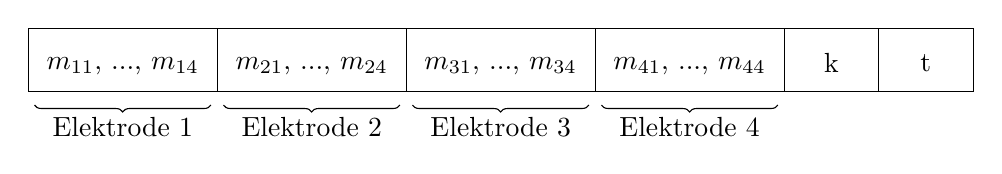
\begin{tikzpicture}[scale=0.8]
		\draw[black, thin] (0,0) rectangle (3,1);
		\draw[decoration={brace,mirror,raise=5pt},decorate]
		(0+0.1,0) -- node[below=6pt] {Elektrode 1} (3-0.1,0);
		
		\draw[black, thin] (3,0) rectangle (6,1);
		\draw[decoration={brace,mirror,raise=5pt},decorate]
		(3+0.1,0) -- node[below=6pt] {Elektrode 2} (6-0.1,0);
		
		\draw[black, thin] (6,0) rectangle (9,1);
		\draw[decoration={brace,mirror,raise=5pt},decorate]
		(6+0.1,0) -- node[below=6pt] {Elektrode 3} (9-0.1,0);
		
		\draw[black, thin] (9,0) rectangle (12,1);
		\draw[decoration={brace,mirror,raise=5pt},decorate]
		(9+0.1,0) -- node[below=6pt] {Elektrode 4} (12-0.1,0);
		
		\draw[black] (12,0) rectangle (13.5,1);
		\draw[black] (13.5,0) rectangle (15,1);

		\node at (0+1.5,0+0.4) {$m_{11}$, ..., $m_{14}$};
		\node at (3+1.5,0+0.4) {$m_{21}$, ..., $m_{24}$};
		\node at (6+1.5,0+0.4) {$m_{31}$, ..., $m_{34}$};
		\node at (9+1.5,0+0.4) {$m_{41}$, ..., $m_{44}$};
		\node at (12+0.75,0+0.45) {k};
		\node at (13.5+0.75,0+0.45) {t};
		\end{tikzpicture}
		\caption{Aufbau eines Eintrags im Datensatz, während $m_{1x}$ das $x$te Merkmal der 1. Elektrode bezeichnet. Die aufgezeichnete Klasse wird durch $k$ und die aktuelle Aufnahmesitzung durch $t$ gekennzeichnet (eigene Darstellung).}
		\label{dataset-item}
	\end{center}
\end{figure}

